\section{Additional Theoretical ICD/ETMD3 Spectra}

\subsection{Clusters with $N=38$ Atoms of Different Composition}

\begin{figure}
 \centering
 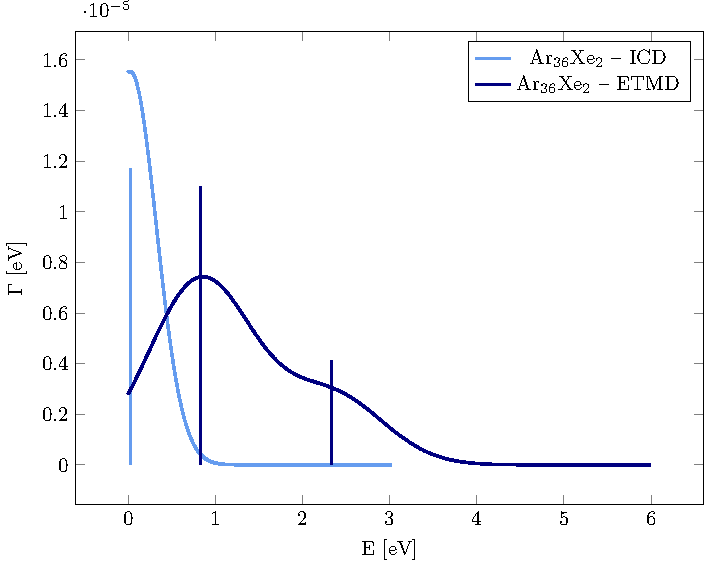
\includegraphics[width=0.5\columnwidth]{pics/Ar36Xe2.pdf}
 \caption{}
 \label{}
\end{figure}


\begin{figure}
 \centering
 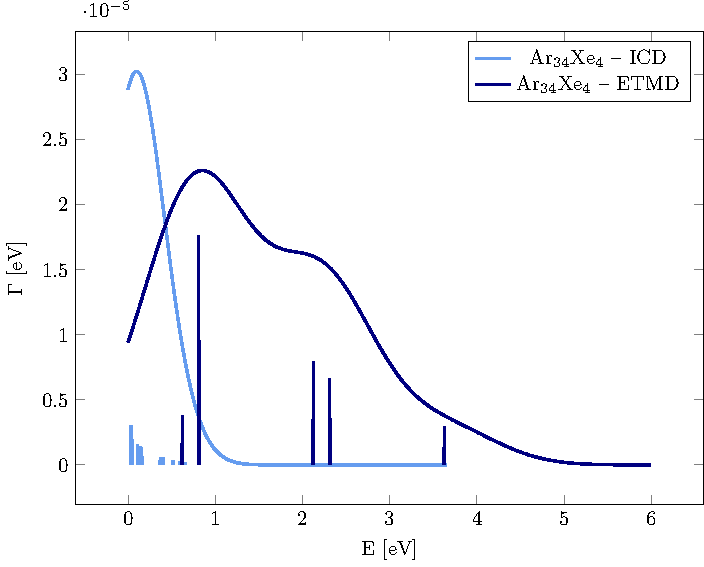
\includegraphics[width=0.5\columnwidth]{pics/Ar34Xe4.pdf}
 \caption{}
 \label{}
\end{figure}


\begin{figure}
 \centering
 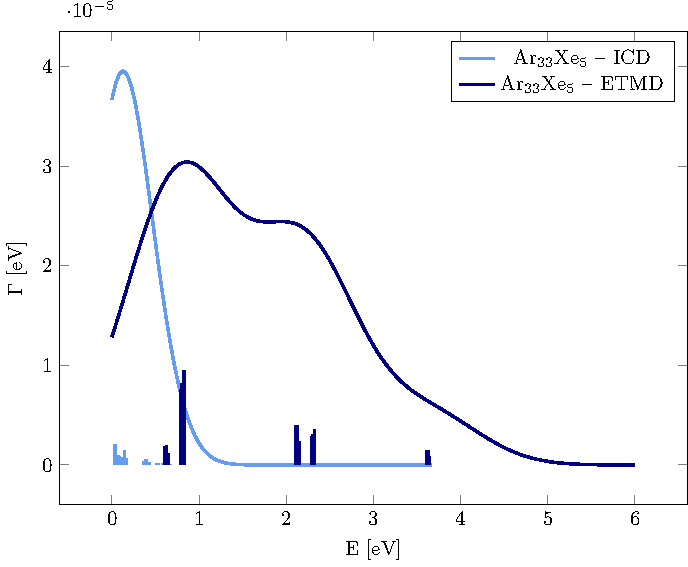
\includegraphics[width=0.5\columnwidth]{pics/Ar33Xe5.pdf}
 \caption{}
 \label{}
\end{figure}

\begin{figure}
 \centering
 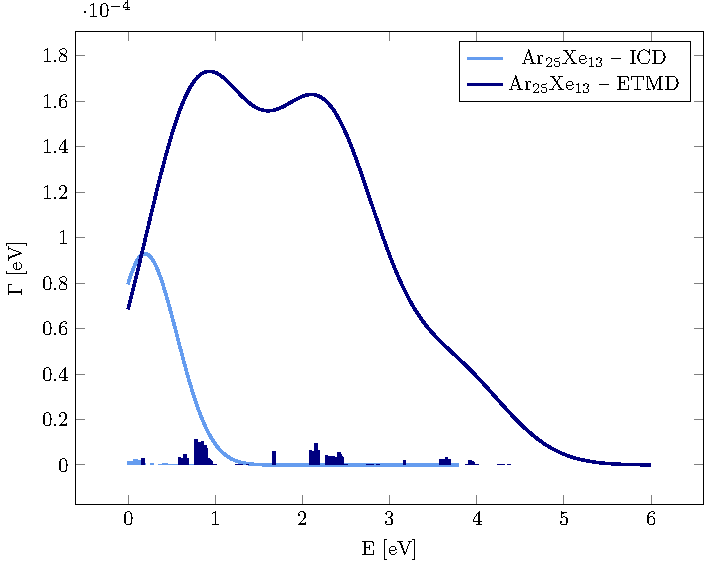
\includegraphics[width=0.5\columnwidth]{pics/Ar25Xe13.pdf}
 \caption{}
 \label{}
\end{figure}

\begin{figure}
 \centering
 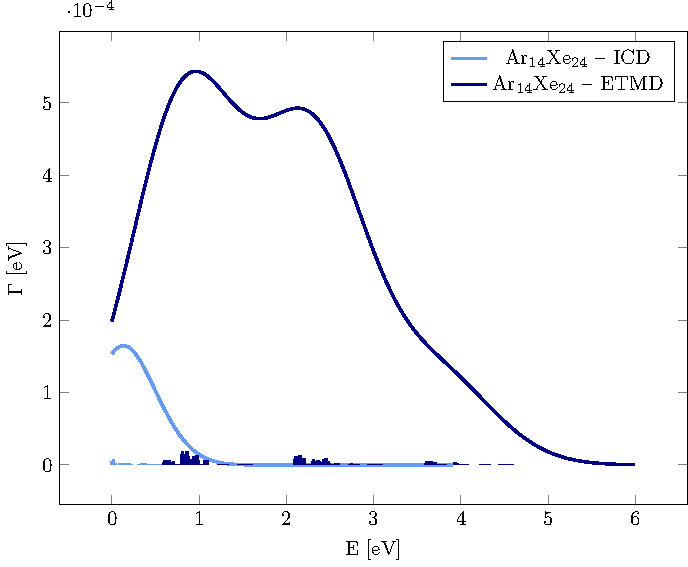
\includegraphics[width=0.5\columnwidth]{pics/Ar14Xe24.pdf}
 \caption{}
 \label{figure:}
\end{figure}

\begin{figure}
 \centering
 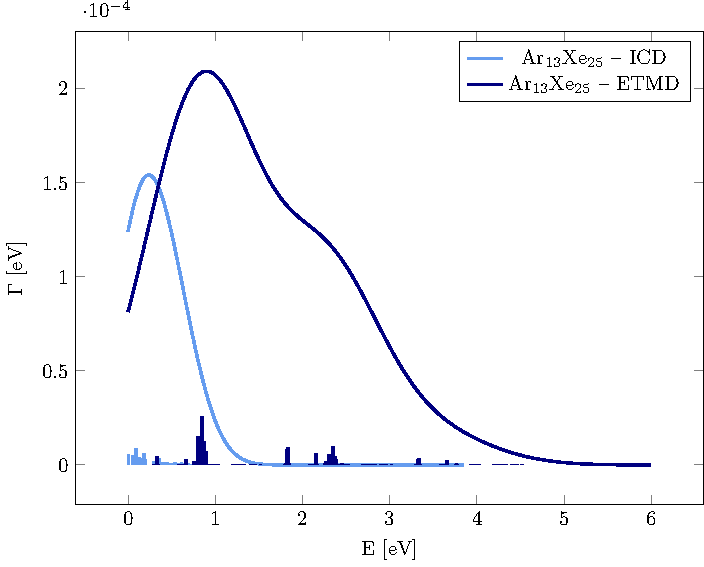
\includegraphics[width=0.5\columnwidth]{pics/Ar13Xe25.pdf}
 \caption{}
 \label{figure:Ar13Xe25}
\end{figure}

\begin{figure}
 \centering
 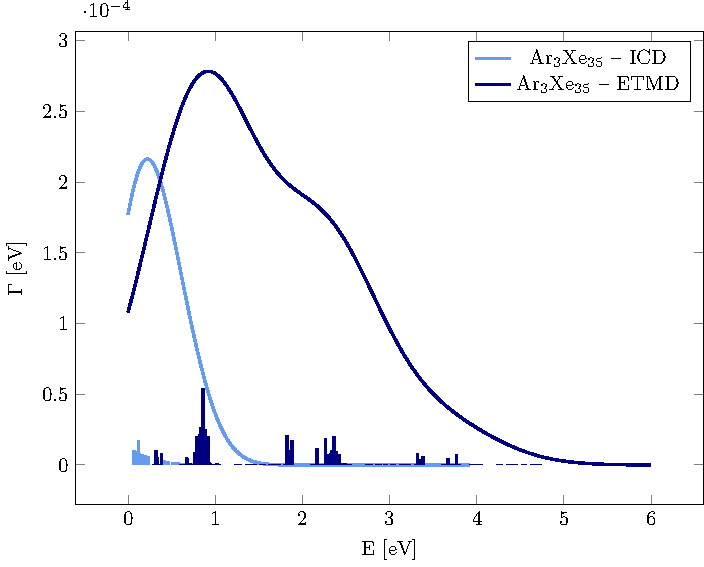
\includegraphics[width=0.5\columnwidth]{pics/Ar3Xe35.pdf}
 \caption{}
 \label{figure:Ar3Xe35}
\end{figure}

%\begin{figure}
% \centering
% \includegraphics[width=0.5\columnwidth]{pics/ArXe.pdf}
% \caption{}
% \label{}
%\end{figure}
%
%\begin{figure}
% \centering
% \includegraphics[width=0.5\columnwidth]{pics/ArXe.pdf}
% \caption{}
% \label{}
%\end{figure}
